%%%%%%%%%%%%%%%%%%%%%%%%%%%%%%%%%%%%%%%%%%%%%%%%%%%%%%
% A Beamer template for University of Wollongong     %
% Based on THU beamer theme                          %
% Author: Qiuyu Lu                                   %
% Date: July 2024                                    %
% LPPL Licensed.                                     %
%%%%%%%%%%%%%%%%%%%%%%%%%%%%%%%%%%%%%%%%%%%%%%%%%%%%%%
% Customized for Sharif University of Technology     %
%%%%%%%%%%%%%%%%%%%%%%%%%%%%%%%%%%%%%%%%%%%%%%%%%%%%%%


\documentclass[serif, aspectratio=169]{beamer}
%\documentclass[serif]{beamer}  % for 4:3 ratio
\usepackage[T1]{fontenc} 
\usepackage{fourier} % see "http://faq.ktug.org/wiki/uploads/MathFonts.pdf" for other options
\usepackage{hyperref}
\usepackage{latexsym,amsmath,xcolor,multicol,booktabs,calligra}
\usepackage{graphicx,pstricks,listings,stackengine}
\usepackage{lipsum}
\usepackage{tikz}
% For writing clean pseudocodes
% \usepackage{algorithm, algpseudocode, mathtools, needspace}
% \usepackage{algorithmic}
\usepackage{algorithm}
\usepackage{algorithmic}
% To justify the items


\author{Ali Sharifi-Zarchi}
% \author{CE Department}
\title{Machine Learning (CE 40477)}
\subtitle{Fall 2024}
\institute{
    CE Department \\
    Sharif University of Technology
}
%\date{\small \today}
% \usepackage{UoWstyle}
\usepackage{SUTstyle}

% defs
\def\cmd#1{\texttt{\color{red}\footnotesize $\backslash$#1}}
\def\env#1{\texttt{\color{blue}\footnotesize #1}}
\definecolor{deepblue}{rgb}{0,0,0.5}
\definecolor{deepred}{RGB}{153,0,0}
\definecolor{deepgreen}{rgb}{0,0.5,0}
\definecolor{halfgray}{gray}{0.55}

\lstset{
    basicstyle=\ttfamily\small,
    keywordstyle=\bfseries\color{deepblue},
    emphstyle=\ttfamily\color{deepred},    % Custom highlighting style
    stringstyle=\color{deepgreen},
    numbers=left,
    numberstyle=\small\color{halfgray},
    rulesepcolor=\color{red!20!green!20!blue!20},
    frame=shadowbox,
}

% For writing comments that are aligned to the left side
\makeatletter
\NewDocumentCommand{\LeftComment}{s m}{%
  \Statex \IfBooleanF{#1}{\hspace*{\ALG@thistlm}}\(\triangleright\) #2}
\makeatother
% To manually indent states in algorithmicx
\newcommand{\IndState}{\State\hspace{\algorithmicindent}}
% To make breakable algorithms
\makeatletter
\newenvironment{nofloatalgorithmic}[2][0]
  {
  \par
  \needspace{\dimexpr\baselineskip+6.8pt}
  \noindent
  \hrule height.8pt depth0pt \kern2pt
  \refstepcounter{algorithm}
  \addcontentsline{loa}{algorithm}{\numberline{\thealgorithm}#2}
  \noindent\textbf{\fname@algorithm~\thealgorithm} #2\par
  \kern2pt\hrule\kern2pt
  \begin{algorithmic}[#1]
  }
  {
  \end{algorithmic}
  \nobreak\kern2pt\hrule\relax
  }
\makeatother
% To make vertical arrow
\newcommand\vertarrowbox[3][6ex]{%
  \begin{array}[t]{@{}c@{}} #2 \\
  \left\uparrow\vcenter{\hrule height #1}\right.\kern-\nulldelimiterspace\\
  \makebox[0pt]{\scriptsize#3}
  \end{array}%
}
% Clean argmin
\DeclareMathOperator*{\argmin}{arg\,min}


\begin{document}

\begin{frame}
    \titlepage
    \vspace*{-0.6cm}
    \begin{figure}[htpb]
        \begin{center}
            
\includegraphics[keepaspectratio, scale=0.25]{pic/sharif-main-logo.png}
        \end{center}
    \end{figure}
\end{frame}

\begin{frame}    
\tableofcontents[sectionstyle=show,
subsectionstyle=show/shaded/hide,
subsubsectionstyle=show/shaded/hide]
\end{frame}

\section{Unsupervised Learning Overview}
\begin{frame}{Unsupervised Learning}
    \textbf{Unsupervised Learning} involves working with \textbf{unlabeled data}, where the goal is to \textbf{infer the natural structure} present within a set of data points.
    \begin{itemize}
        \item Learning from unlabeled data.
        \item Most of the times, there is no (or minimal) prior knowledge of the data.
        \item Two of the most common techniques:
        \begin{itemize}
            \item \textbf{Clustering}: Grouping data points into clusters based on similarity towards user need.
            \item \textbf{Dimensionality Reduction}: Reducing the number of features under consideration and keeping (perhaps approximately) the most informative features.
        \end{itemize}
    \end{itemize}
\end{frame}

\begin{frame}{Clustering: Bio-informatics}
    \begin{figure}
        \centering
        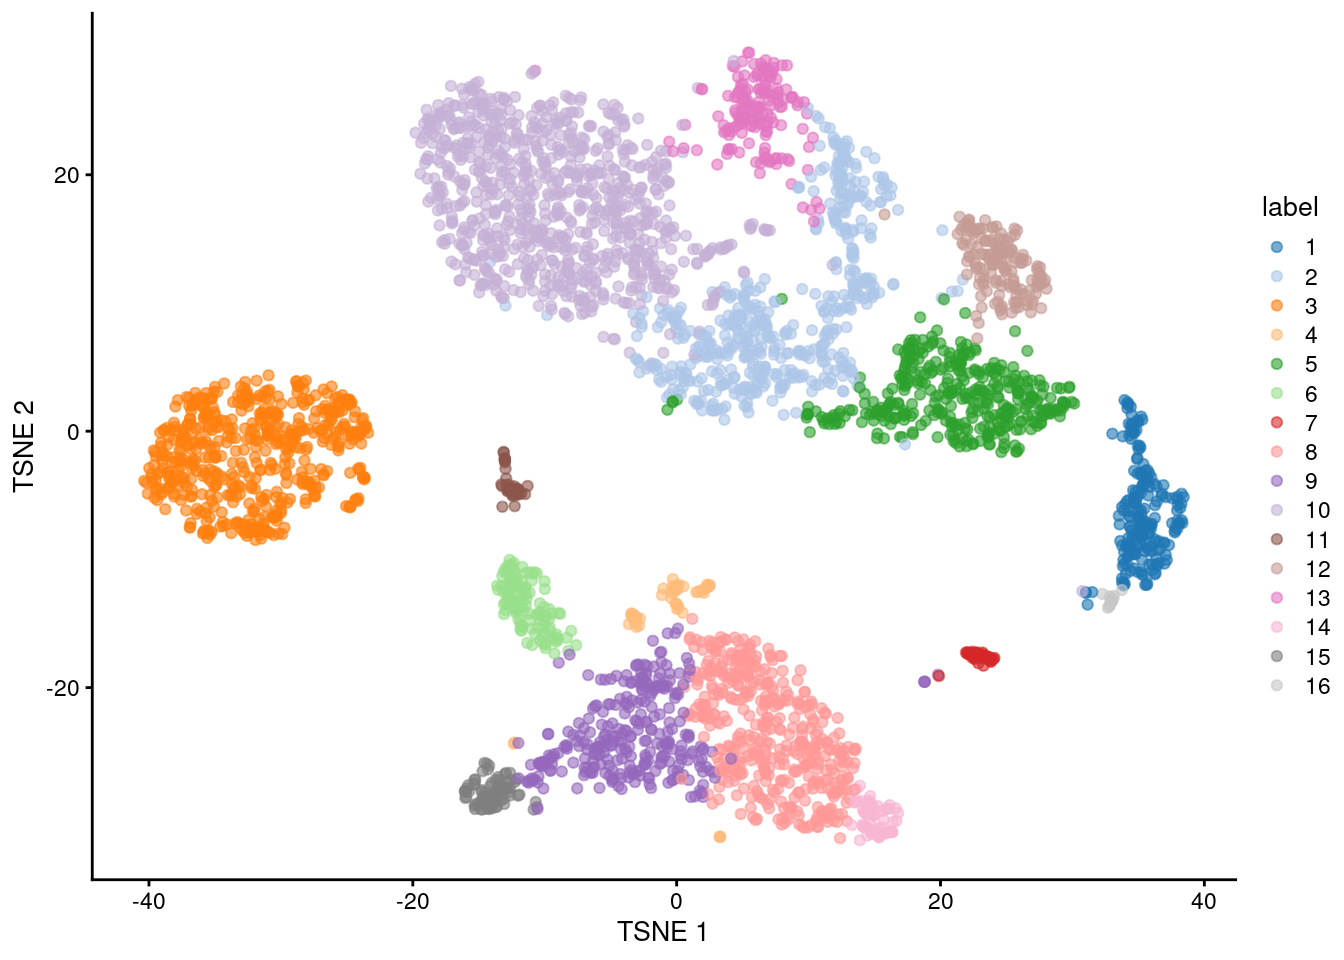
\includegraphics[scale=0.5]{pic/bioconductor_clustering.png}
    \end{figure}
        \begin{tikzpicture}[remember picture,overlay]
        \node[anchor=south west, xshift=0.1cm, yshift=0.22cm] at (current page.south west) {
            \scriptsize Figure adapted from \href{https://bioconductor.org/books/3.15/OSCA.basic/clustering.html}{bioconductor.org}
        };
    \end{tikzpicture}
\end{frame}

\begin{frame}{Slide showcasing reduction (PCA)}
    
\end{frame}

\begin{frame}{Clustering: Customer segmentation}
    \begin{figure}
        \centering
        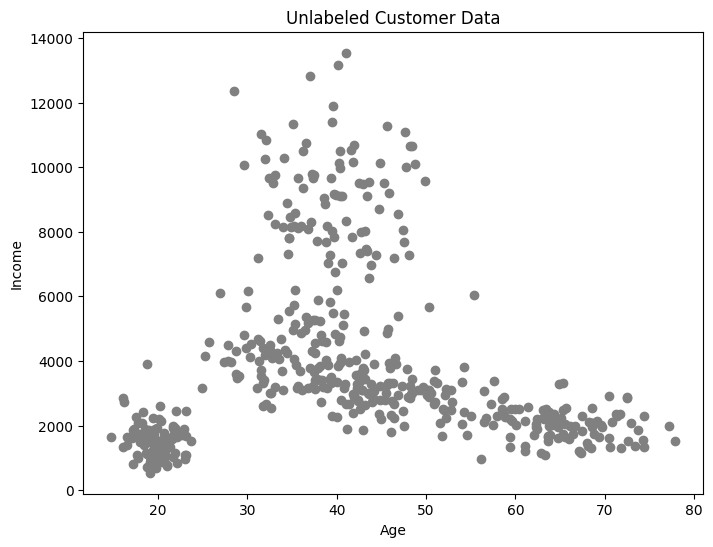
\includegraphics[scale=0.45]{pic/customer_clusters_raw_plot.png}
    \end{figure}
    \begin{center}
        Information of customers
    \end{center}
\end{frame}

\begin{frame}{Clustering: Customer segmentation (cont.)}
    \begin{figure}
        \centering
        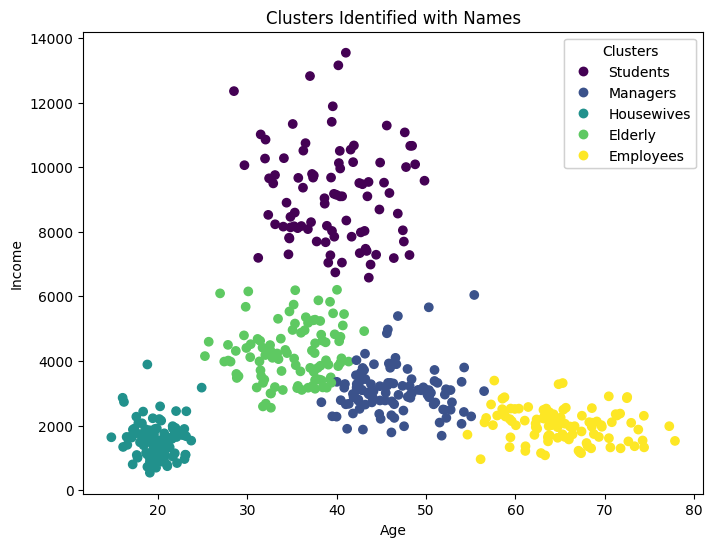
\includegraphics[scale=0.45]{pic/customer_clusters.png}
    \end{figure}
    \begin{center}
        Predicted clusters of customers
    \end{center}
\end{frame}

\section{Clustering}

\begin{frame}{Clustering}
    \begin{minipage}{0.95\textwidth}
        \begin{itemize}
        \item Assume we have a set of unlabeled data points $ \{ \mathbf{x}^{(i)} \}_{i=1}^N$.
        \item We intend to find \textbf{groups of similar objects} with respect to our need.
        \begin{itemize}
            \item For example all data points having most similar number of buys in a market.
        \end{itemize}
        \item It helps us to gain insight into structure of data prior to class design.
        \item Clustering could also help to compress and reduce data.
    \end{itemize}
    \end{minipage}%
    % \begin{minipage}{0.45\textwidth}
    %     \begin{itemize}
    %     \item Assume we have a set of unlabeled data points $ \{ \mathbf{x}^{(i)} \}_{i=1}^N$.
    %     \item We intend to find \textbf{groups of similar objects} with respect to our need.
    % \end{itemize}
    % \end{minipage}
\end{frame}

\begin{frame}{Clustering (cont.)}
    \begin{minipage}{0.55\textwidth}
        From another point of view, clusters are regions of high density that are separated from one another with regions of low density.
    % here we should talk what is good cluster ? should we even try to cluster based on density function ? should we focus of pure samples ? showcase the problem in which clustering could be both circle and a line extending of pmf (or pdf)
    \end{minipage}%
    \begin{minipage}{0.4\textwidth}
        \begin{figure}
            \centering
            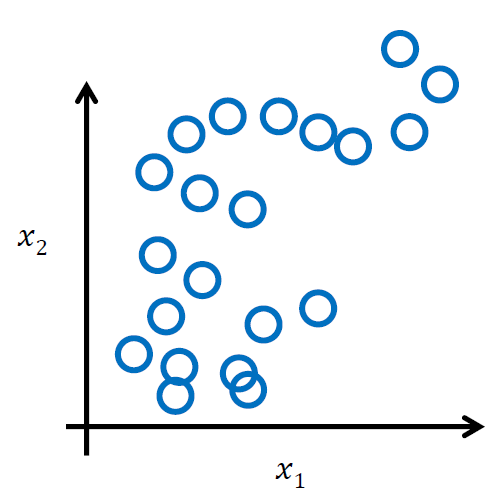
\includegraphics[scale=0.5]{pic/clusteriong_pov.png}
        \end{figure}
    \end{minipage}
    \begin{tikzpicture}[remember picture,overlay]
        \node[anchor=south west, xshift=0.1cm, yshift=0.22cm] at (current page.south west) {
            \scriptsize Figure adapted from slides of Dr. Soleymani, Machine Learning course, Sharif University of technology.
        };
    \end{tikzpicture}
\end{frame}

\begin{frame}{Hard clustering vs Soft clustering}
    \begin{minipage}{0.55\textwidth}
        \begin{itemize}
        \item \textbf{Hard Clustering:} Each data point belongs to exactly one cluster
        \begin{itemize}
            \item more common and easier to do
        \end{itemize}
        \item \textbf{Soft Clustering}
    \end{itemize}
    \end{minipage}%
    \begin{minipage}{0.40\textwidth}
        \begin{figure}
            \centering
            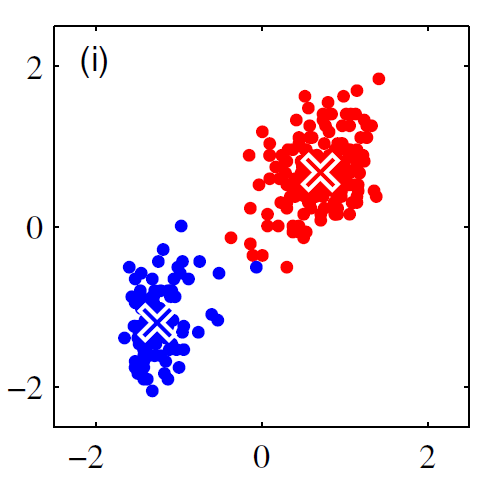
\includegraphics[scale=0.5]{pic/hard_clustering.png}
        \end{figure}
    \end{minipage}
    \begin{tikzpicture}[remember picture,overlay]
        \node[anchor=south west, xshift=0.1cm, yshift=0.22cm] at (current page.south west) {
            \scriptsize Figure adapted from Machine Learning and Pattern Recognition, Bishop
        };
    \end{tikzpicture}  
\end{frame}

\begin{frame}{Hard clustering vs Soft clustering (cont.)}
    \begin{minipage}{0.55\textwidth}
        \begin{itemize}
        \item \textbf{Hard Clustering}
        \item \textbf{Soft Clustering:} Each data point can belong to multiple clusters.
        \begin{itemize}
            \item data point belongs to each cluster with a probability
        \end{itemize}
        \item \textbf{From now on, we will focus on problem of hard clustering}
    \end{itemize}
    \end{minipage}%
    \begin{minipage}{0.40\textwidth}
        \begin{figure}
            \centering
            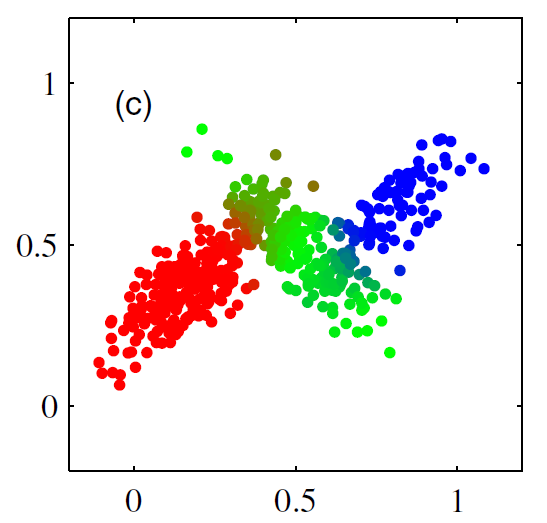
\includegraphics[scale=0.5]{pic/soft_clustering.png}
        \end{figure}
    \end{minipage}
    \begin{tikzpicture}[remember picture,overlay]
        \node[anchor=south west, xshift=0.1cm, yshift=0.22cm] at (current page.south west) {
            \scriptsize Figure adapted from Machine Learning and Pattern Recognition, Bishop
        };
    \end{tikzpicture}  
\end{frame}

\begin{frame}{Hard clustering problem}
    \begin{itemize}
        \item We need to \textbf{partition} \( N \) data points to \( K \) clusters.
        \item Good flat clustering should have two important factors:
        \begin{itemize}
            \item Data points in a cluster should be similar (\textbf{High intra-cluster similarity})
            \item Data points in different clusters should be less similar (\textbf{Low inter-cluster similarity})
        \end{itemize}
        \item As mentioned earlier, each partitional clustering method requires a \textbf{similarity metric} between data points.
    \end{itemize}
\end{frame}

\begin{frame}{Similarity measure and Distance measure}
    \begin{minipage}{0.6\textwidth}
        \begin{itemize}
            \item Similarity measures are used to distinguish between similar and non-similar data points.
            \item We usually define similarity of two data point as \textbf{inverse of distance} between them.
            \item Using this definition, {hard clustering aims to put data points with less distance in same cluster.}
        \end{itemize}
    \end{minipage}%
    \begin{minipage}{0.35}
        \begin{figure}
            \centering
            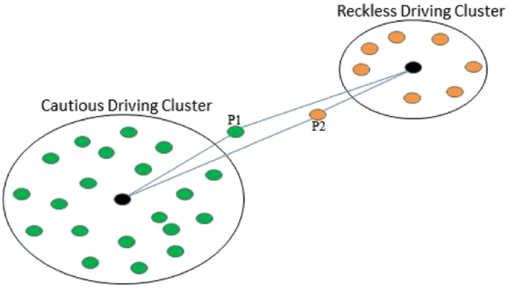
\includegraphics[scale=0.4]{pic/Distance-based-clustering-approach.png}
        \end{figure}
    \end{minipage}
\end{frame}

\begin{frame}{Common similarity and distance measures}
    \begin{itemize}
        \item Assume \( p \) and \( q \) are two data points from $ \mathbb{R}^D$. most common similarity and distance measures in the problem of clustering are as follows:
        \begin{itemize}
            \item \textbf{Euclidean distance:} Most common measure of distance between two vectors doesn't matter.
            \[
            d^2(p,q)=\sqrt{{\sum_{i=1}^{D}{(p_i-q_i)^2}}}
            \]
            \item \textbf{Cosine similarity:} Most common measure of similarity when the magnitude of vectors does not change the similarity
            \[
            \textbf{similarity(\(p\),\(q\))}=\frac{p^T q}{||p|| \ . \ ||q||}
            \]
            \item \textbf{Manhattan distance:} Most common measure of distance when dimensions are not equally important
            \[
            d^2(p,q)=\sqrt{\sum_{i=1}^{D} |p_i-q_i|}
            \]
        \end{itemize}
    \end{itemize}
\end{frame}

\section{K-Means}
\begin{frame}{K-Means overview}
    \begin{itemize}
        \item One of the most common partitional clustering methods used
        \item The idea is to \textbf{find} \( \mathbf{K} \) \textbf{centers.} \textbf{Each center representing a cluster.}
        \item Each data point is assigned to cluster \( j \) if and only if it has the least distance to center of cluster \( j \) amongst all clusters.
        \item K-Means suggest an \textbf{iterative algorithm} to find these centers.
    \end{itemize}
\end{frame}

\begin{frame}{K-Means Clustering}
    \begin{itemize}
        \item \textbf{Input:} a set \( \mathbf{x}^{(1)}, \mathbf{x}^{(2)}, \dots, \mathbf{x}^{(N)} \) of data points (\( \forall x^{(i)} \in \mathbb{R}^D \) and an integer \( K \)
        \item \textbf{Output:} a set of \( K \) representatives \( \mathbf{c}_1, \mathbf{c}_2, \dots, \mathbf{c}_K \) as the cluster representatives
        \begin{itemize}
            \item data points are assigned to the clusters according to their distance to \(\mathbf{c}_1, \mathbf{c}_2, \dots, \mathbf{c}_K \)
            \item each data is assigned to the cluster whose representative is nearest to it
        \end{itemize}
        \item \textbf{Objective:} choose \( \mathbf{c}_1, \mathbf{c}_2, \dots, \mathbf{c}_K \) as to minimize intra-cluster similarity:
        \[
            \sum_{i=1}^{N} min_{j \in 1,2,\dots, K} d^2 \left( \mathbf{x}^{(i)}, \mathbf{c_j} \right)
        \]
    \end{itemize}
\end{frame}

\begin{frame}{K-Means Clustering (cont.)}
    \begin{itemize}
        \item K-Means uses \textbf{Euclidean Distance} measure thus we can rewrite the objective as follows:
        \[
        J\left( \mathbf{c}_1, \mathbf{c}_2, \dots, \mathbf{c}_K \right) = \sum_{i=1}^{N} min_{j \in 1,2,\dots, K} \left| \left| \mathbf{x}^{(i)} - \mathbf{c}_j \right|\right|^2
        \]
        \item This objective function is sometimes called \textbf{distortion} as well.
    \end{itemize}
\end{frame}

\begin{frame}{K-Means Clustering (cont.)}
    \begin{itemize}
        \item \textbf{Why the idea of minimizing distortion works ?}
        \begin{itemize}
            \item Distortion is used to model intra-cluster similarity score. If we can show that \( J( \mathbf{c}_1, \mathbf{c}_2, \dots, \mathbf{c}_K ) \) is optimizable, we can get suggest K-Means actually works.
            \item We just have to make sure each iteration of reaching optimum centers, is decreasing distortion. (or at least doesn't increase it)
            \item Then simply use optimization methods to reach optimum or at least, get as close as possible to it.
        \end{itemize}
    \end{itemize}
\end{frame}

\begin{frame}{K-Means pseudo-code}
    \begin{algorithm}[H]
    \caption{K-Means}\label{alg:K-Means}
    \begin{algorithmic}[1]
    \STATE Select $k$ random points $c_1, c_2, \ldots, c_k$ as clusters' initial centroids 
    \REPEAT 
    \FOR{each $i = 1$ to $N$}
        \STATE Assign $x^{(i)}$ to the closest cluster $C_j$ such that $C_j$ contains all data that are closer to $c_j$ than to any other cluster.
    \ENDFOR
    \FOR{each $j = 1$ to $k$}
        \STATE $c_j = \frac{1}{|C_j|} \sum_{x^{(i)} \in C_j} x^{(i)}$
    \ENDFOR
    \UNTIL{the centroids no longer change}
    \end{algorithmic}
    \end{algorithm}
\end{frame}

\begin{frame}{K-Means pseudo-code (cont.)}
    \begin{itemize}
        \item It is notable that K-Means follows the following two steps until reaching the best clustering status:
        \begin{enumerate}
            \item \textbf{Assigning data points to the closest cluster}
            \item \textbf{Computing new center for each cluster}
        \end{enumerate}
    \end{itemize}
\end{frame}

% K means in action
\begin{frame}{K-Means in action}
    \begin{figure}
        \centering
        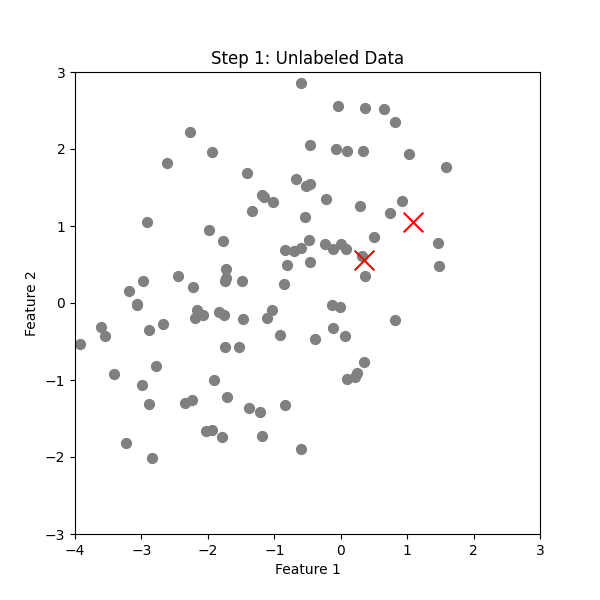
\includegraphics[scale=0.45]{pic/figs/kmeans_step_1_unlabeled_data.png}
    \end{figure}
\end{frame}
\begin{frame}{K-Means in action (cont.)}
    \begin{figure}
        \centering
        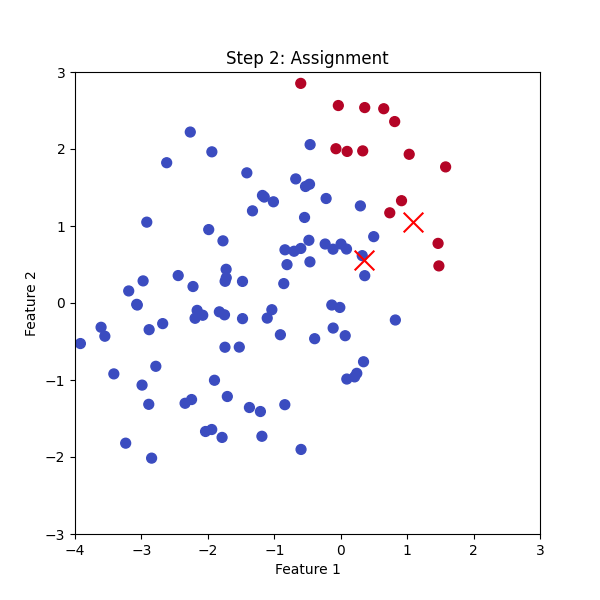
\includegraphics[scale=0.45]{pic/figs/kmeans_step_2_assignment.png}
    \end{figure}
\end{frame}

\begin{frame}{K-Means in action (cont.)}
    \begin{figure}
        \centering
        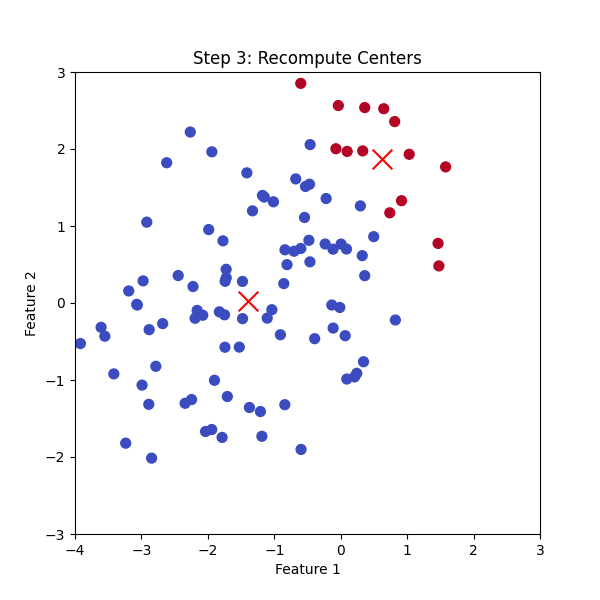
\includegraphics[scale=0.45]{pic/figs/kmeans_step_3_recompute_centers.png}
    \end{figure}
\end{frame}
\begin{frame}{K-Means in action (cont.)}
    \begin{figure}
        \centering
        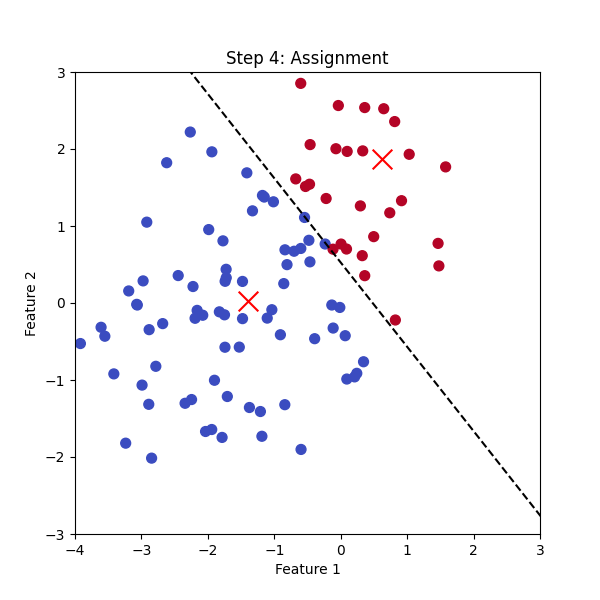
\includegraphics[scale=0.45]{pic/figs/kmeans_step_4_assignment.png}
    \end{figure}
\end{frame}
\begin{frame}{K-Means in action (cont.)}
    \begin{figure}
        \centering
        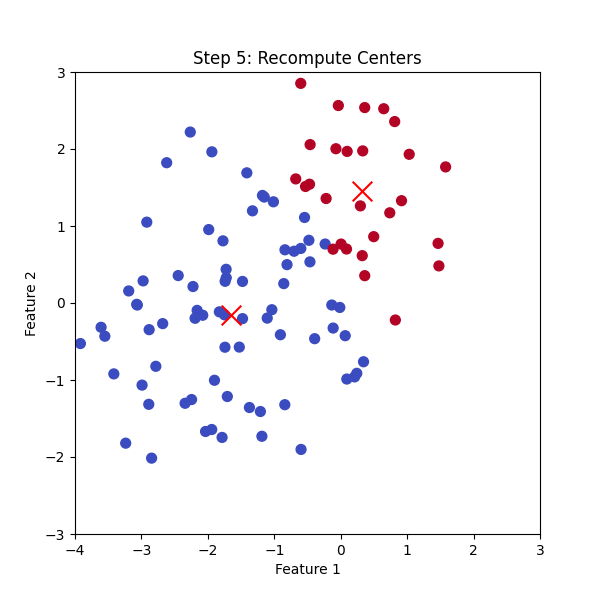
\includegraphics[scale=0.45]{pic/figs/kmeans_step_5_recompute_centers.png}
    \end{figure}
\end{frame}
\begin{frame}{K-Means in action (cont.)}
    \begin{figure}
        \centering
        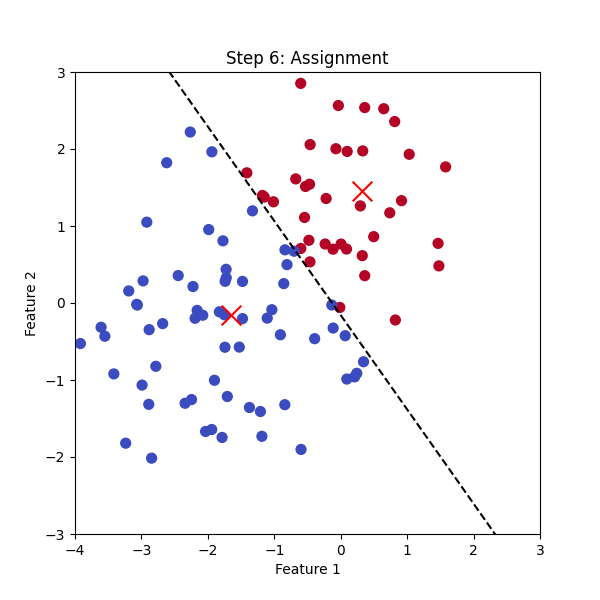
\includegraphics[scale=0.45]{pic/figs/kmeans_step_6_assignment.png}
    \end{figure}
\end{frame}
\begin{frame}{K-Means in action (cont.)}
    \begin{figure}
        \centering
        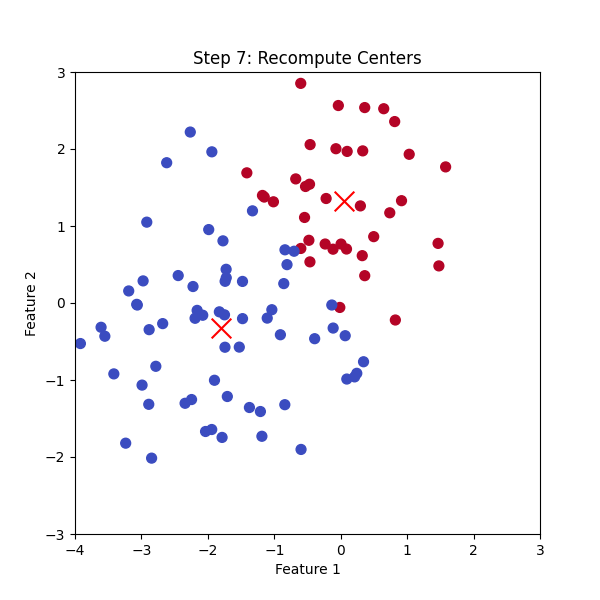
\includegraphics[scale=0.45]{pic/figs/kmeans_step_7_recompute_centers.png}
    \end{figure}
\end{frame}
\begin{frame}{K-Means in action (cont.)}
    \begin{figure}
        \centering
        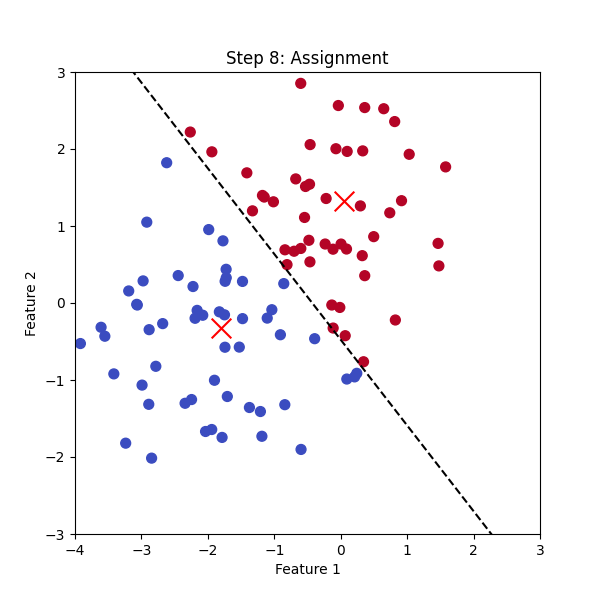
\includegraphics[scale=0.45]{pic/figs/kmeans_step_8_assignment.png}
    \end{figure}
\end{frame}
\begin{frame}{K-Means in action (cont.)}
    \begin{figure}
        \centering
        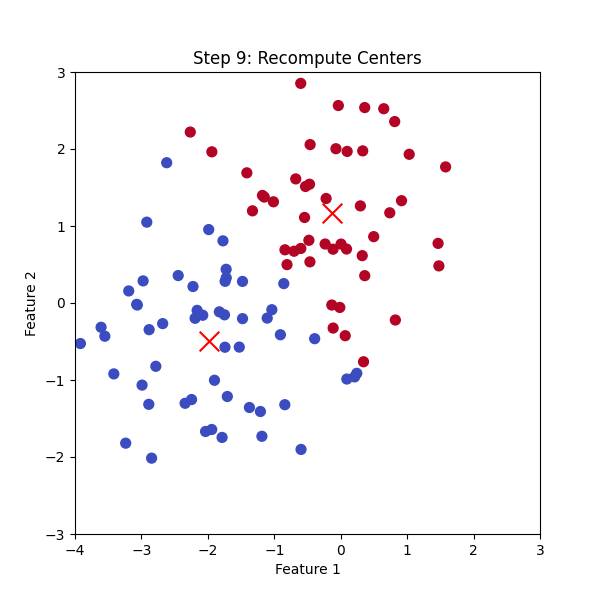
\includegraphics[scale=0.45]{pic/figs/kmeans_step_9_recompute_centers.png}
    \end{figure}
\end{frame}
\begin{frame}{K-Means in action (cont.)}
    \begin{figure}
        \centering
        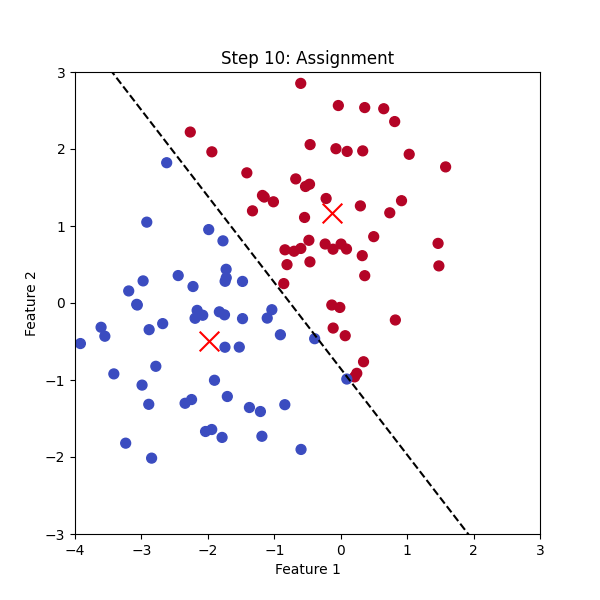
\includegraphics[scale=0.45]{pic/figs/kmeans_step_10_assignment.png}
    \end{figure}
\end{frame}
\begin{frame}{K-Means in action (cont.)}
    \begin{figure}
        \centering
        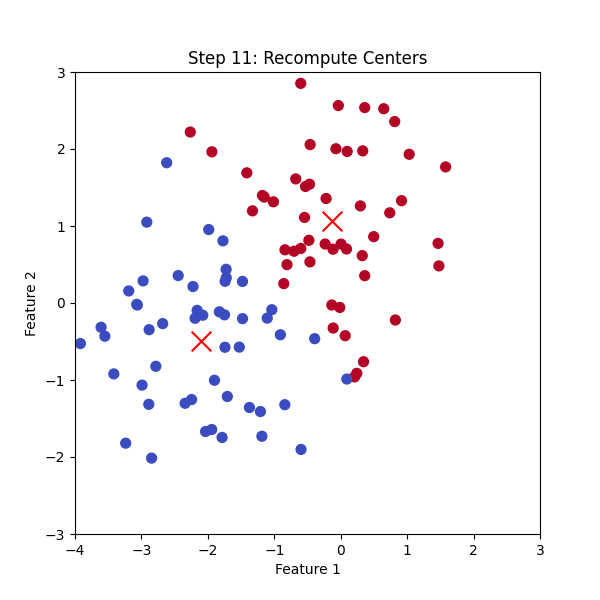
\includegraphics[scale=0.45]{pic/figs/kmeans_step_11_recompute_centers.png}
    \end{figure}
\end{frame}
\begin{frame}{K-Means in action (cont.)}
    \begin{figure}
        \centering
        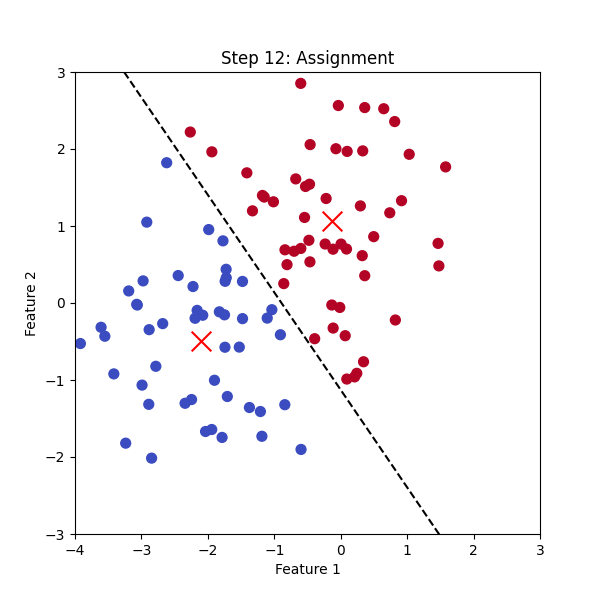
\includegraphics[scale=0.45]{pic/figs/kmeans_step_12_assignment.png}
    \end{figure}
\end{frame}
\begin{frame}{K-Means in action (cont.)}
    \begin{figure}
        \centering
        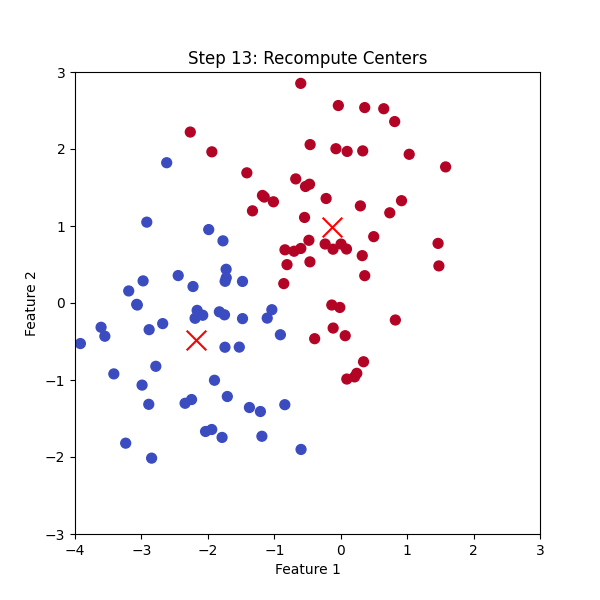
\includegraphics[scale=0.45]{pic/figs/kmeans_step_13_recompute_centers.png}
    \end{figure}
\end{frame}
\begin{frame}{K-Means in action (cont.)}
    \begin{figure}
        \centering
        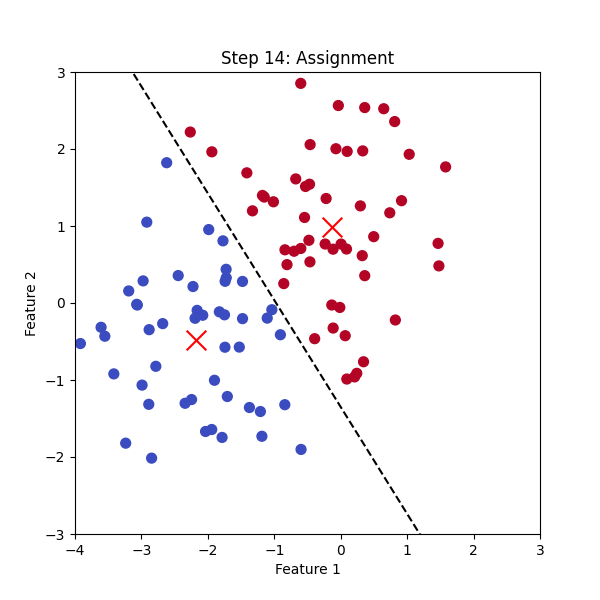
\includegraphics[scale=0.45]{pic/figs/kmeans_step_14_assignment.png}
    \end{figure}
\end{frame}

\begin{frame}{Steps of K-Means}
    \begin{itemize}
        \item \textbf{Why the steps of K-Means have been chosen as explained ?}
        \item Let us rewrite distortion as follows:
        \[ 
        J(\mathbf{c}_1, \mathbf{c}_2, \dots, \mathbf{c}_K) = \sum_{i=1}^{N} \sum_{j=1}^{K} r_{ij} \ || \mathbf{x}^{(i)} - \mathbf{c}_j ||^2
        \]
        \item In which \( r_{ij} \) is an indicator defined as:
        \begin{center}
        \( r_{ij} = \)
        \begin{cases}
        1 \ \ \ \ \mathbf{x}^{(i)} \\ is \ \ assigned \ \ to \ \ cluster \ \ j\\
        0 \ \ \ \ o.w.
        \end{cases}
        \end{center}
    \end{itemize}
\end{frame}

\begin{frame}{Steps of K-Means (cont.)}
    \begin{itemize}
        \item Let us first assume \( K \) centers are fixed. We need to optimize \( J \) with respect to \( r_{ij} \).
        \item Because \( J \) is a linear function of \( r_{ij} \), this optimization can be performed easily to give a closed form solution. 
        \item The terms involving different n are independent and so we can optimize for each \(n\) separately by choosing \(r_{ij}\) to be 1 for whichever value of k gives the minimum value of \( || \mathbf{x}^{(i)} - \mathbf{c}_j || \)
        \item \(r_{ij}\) can be written as follows:
        \begin{center}
        \( r_{ij} = \)
        \begin{cases}
        1 \ \ \ \ if \ \ j = arg \ min_j \ || \mathbf{x}^{(i)} - \mathbf{c}_j || \\
        0 \ \ \ \ o.w.
        \end{cases}
        \end{center}
    \end{itemize}
\end{frame}

\begin{frame}{Steps of K-Means (cont.)}
    \begin{itemize}
        \item Now let us assume one step of assignment has been performed. We need to optimize \( J \) with respect to \( \mathbf{c}_1, \mathbf{c}_2, \dots, \mathbf{c}_K \)
        \item Objective function \( J \) is quadratic with respect to each \( \mathbf{c}_j \), thus can be solved by setting it's partial derivatives equal to zero:
        \[ 
        \frac{\partial J}{\partial \mathbf{c}_j} = 0 \implies 2 \sum_{i=1}^{N} r_{ij} \left(\mathbf{x}^{(i)} - \mathbf{c}_j \right) = 0
        \]
        \item Solving the equations above gives us:
        \[ 
        \mathbf{c}_j = \frac{\sum_{i=1}^{N}{r_{ij}\mathbf{x}^{(i)}}}{\sum_{i=1}^{N} r_{ij}}
        \]
    \end{itemize}
\end{frame}

\begin{frame}{k-Means convergence}
    \begin{itemize}
        \item It always converges.
        \item Why should the K-Means algorithm ever reach a state in which clustering doesn't change ?
        \begin{itemize}
            \item We have shown reassignment step monotonically decreases \( J \) since each data point is assigned to the nearest cluster.
            \item We have also proven center updates also minimizes sum of squared distances of the assigned data points to the cluster from its center.
        \end{itemize}
    \end{itemize}
\end{frame}
\begin{frame}{K-Means convergence (cont.)}
    \begin{figure}
        \centering
        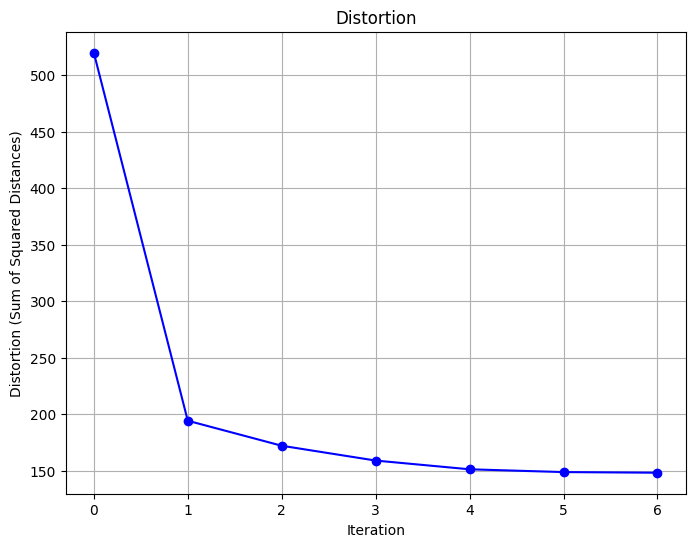
\includegraphics[scale=0.45]{pic/figs/distortion.png}
    \end{figure}
\end{frame}

\begin{frame}{Local optimum}
    \begin{itemize}
        \item k-Means always converges.
        \item However; it may converge at local optimum that is different from the global optimum in terms of objective score.
        \begin{figure}
            \centering
            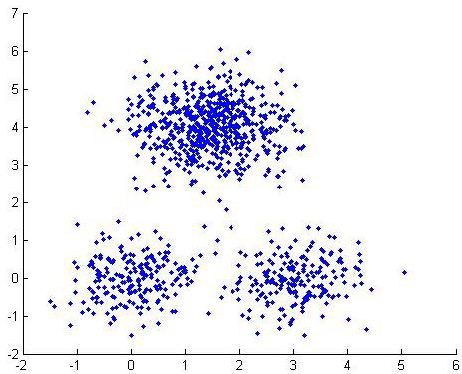
\includegraphics[scale=0.55]{pic/original_data.png}
        \end{figure}
    \end{itemize}
\end{frame}
\begin{frame}{Local optimum (cont.)}
    \begin{minipage}{0.5\textwidth}
        \begin{figure}
            \centering
            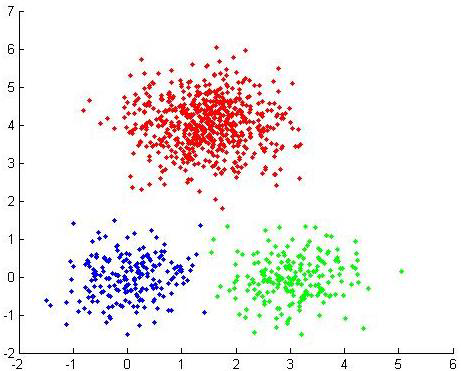
\includegraphics[scale=0.55]{pic/optimal_clustering.png}
        \end{figure}
        \vfill
        \begin{center}
            Optimal clustering
        \end{center}
    \end{minipage}%
    \begin{minipage}{0.5\textwidth}
        \begin{figure}
            \centering
            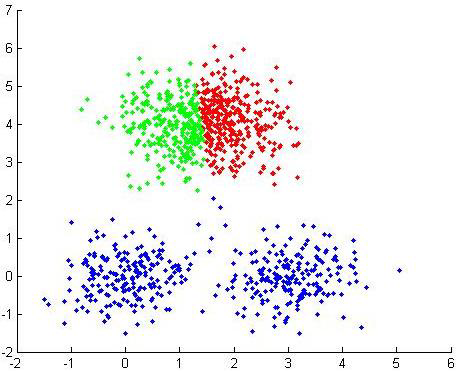
\includegraphics[scale=0.55]{pic/possible_clustering.png}
        \end{figure}
        \vfill
        \begin{center}
            Possible clustering
        \end{center}
    \end{minipage}
\end{frame}

\begin{frame}{K-Means limitations}
    \begin{itemize}
        \item Initialization is crucial as it can determine how fast the algorithm converges.
        \item To overcome the problem of local minima, there are numerous solutions:
        \begin{itemize}
            \item Selecting random centers from data points
            \item Initialize with the suggested results of another method
            \item Use heuristics to find good initial centers 
            \begin{itemize}
                \item K-Means++
                \item Furthest point
            \end{itemize}
        \end{itemize}
        \item Often, k-Means fails to find clusters of arbitary shapes and sizes.
        \begin{itemize}
            \item Except to very distant clusters.
        \end{itemize}
    \end{itemize}
\end{frame}

\begin{frame}{How many clusters?}
    \begin{figure}
        \centering
        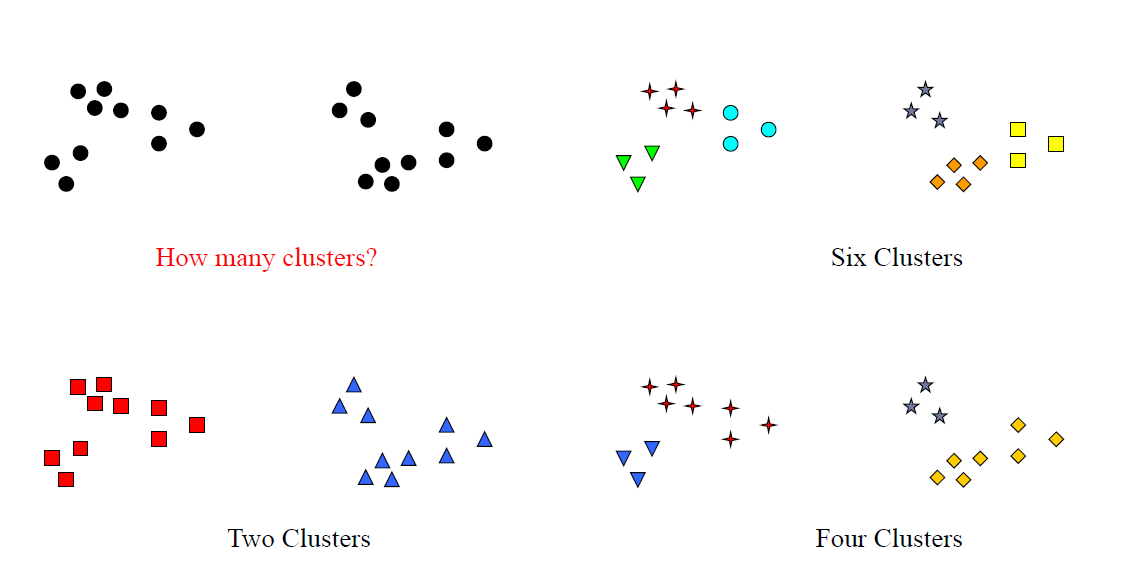
\includegraphics[scale=0.5]{pic/how_many_clusters.png}
    \end{figure}
    \begin{tikzpicture}[remember picture,overlay]
        \node[anchor=south west, xshift=0.1cm, yshift=0.22cm] at (current page.south west) {
            \scriptsize Figure adapted from slides of Dr. Soleymani, Modern Information Retrieval Course, Sharif University of technology.
        };
    \end{tikzpicture}
\end{frame}

\begin{frame}{How many clusters? (cont.)}
    \begin{itemize}
        \item Number of clusters is given in advance in the problem of clustering. However; finding the \textbf{right} number of clusters is also a problem.
        \item There is a tradeoff between having better focus within each cluster or having too many clusters.
        \item \textbf{Optimization problem:} penalize having too much clusters
        \begin{itemize}
            \item Application dependent
        \end{itemize}
        \[
        K^* = \ arg \ min_k \  J(k) + \lambda k 
        \]
    \end{itemize}
\end{frame}

% \begin{frame}{others}
%     How do you find optimal K? (Is the elbow informative?)
% Outliers and pointless clusters and introducing k-means++
% Unknown number of clusters (regularization)
% External clustering criteria (purity, r-index, NMI, F-measure)

% \end{frame}

\begin{frame}{External criteria}
    External clustering criteria (purity, r-index, NMI, F-measure)
\end{frame}

\section{References}

\begin{frame}{Contributions}
\begin{itemize}
\item \textbf{This slide has been prepared thanks to:}
\begin{itemize}
    % \setlength{\itemsep}{10pt} % Adjust the value to control the spacing
    % \item \href{https://github.com/Mahan-Bayhaghi}{Mahan Bayhaghi}
\end{itemize}
\end{itemize}

\end{frame}

\begin{frame}[allowframebreaks]
    \bibliography{ref}
    \bibliographystyle{ieeetr}
    \nocite{*}
\end{frame}

\end{document}